\subsection{Light Pseudoscalar Mesons} 
The following analysis will concentrate on the lightest neutral pseudoscalar meson, $\pi^0$, which is member of the family of $P_p$($\pi^{0}, \eta, \eta'$)($J^{P}=0^{-}$) mesons that are subject to U(3) flavor symmetry. The nonet, the resulting nine states that can be decomposed into a singlet and an octet state, of the pseudoscalar mesons are seen in Fig.~\ref{fig:nonet.pseud}, where strangeness increases upward on the page and charge increases toward the right side of the page.
\begin{figure}[h!]\begin{center}
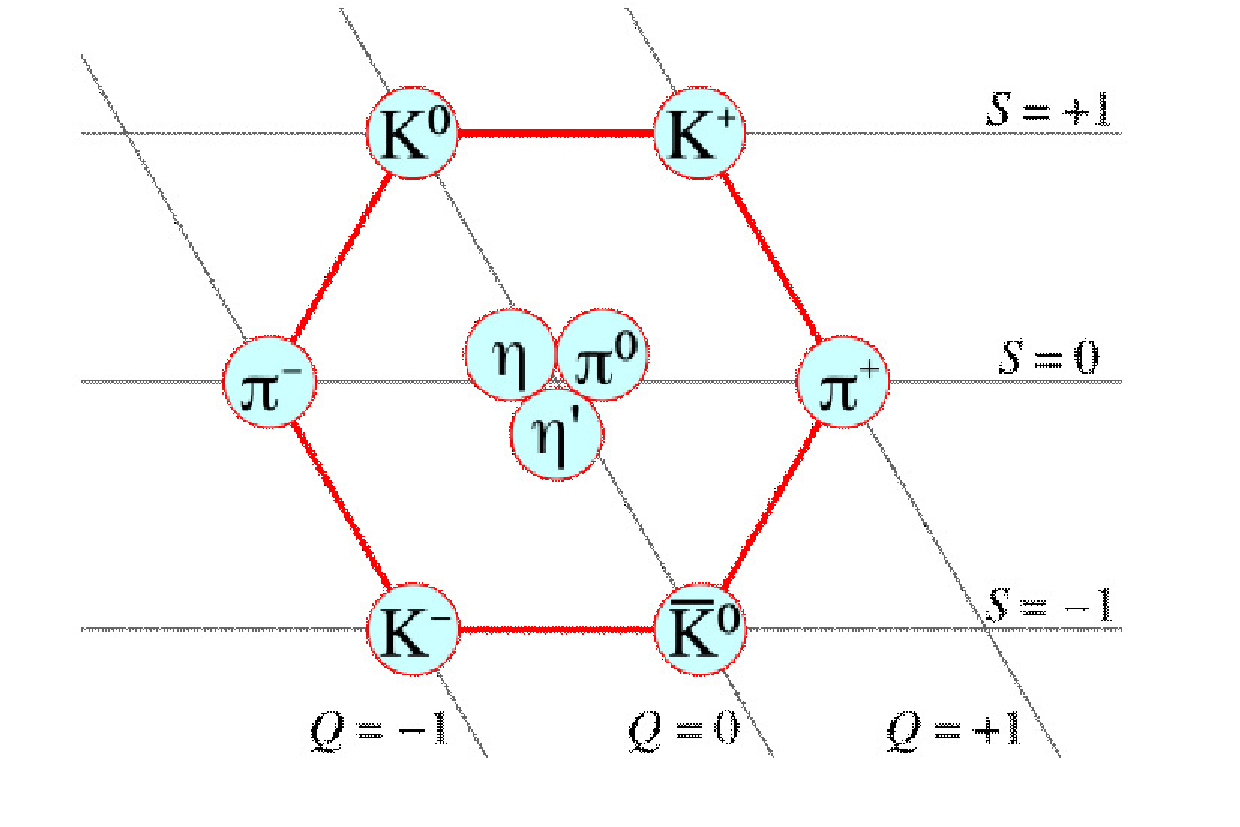
\includegraphics[width= 0.8 \figwidth ,height=\qfigheight]{\grpath/intro/pseudoscalar.pdf}
\caption[Nonet of Pseudoscalar Mesons]{\label{fig:nonet.pseud}Nonet of Pseudoscalar Mesons~\cite{wiki1}.}
\end{center}\end{figure}
It should be noted that the $\eta$ and $\eta'$ are not exact octet ($\eta_{8}$) and singlet ($\eta_{0}$) states, as they are linear combinations of $\eta_{8}$ and $\eta_{0}$ according to:
\begin{eqnarray}
\left(
\begin{array}{cc}
\eta \\
\eta ' 
\end{array}
\right)
& = &
\left(
\begin{array}{cc}
-\sin\theta_{mix} & \cos\theta_{mix} \\
\cos\theta_{mix} & \sin\theta_{mix}
\end{array}
\right)
\cdot
\left(
\begin{array}{cc}
\eta_{0} \\
\eta_{8}
\end{array}
\right)
\end{eqnarray}
where $\theta_{mix} = -18.6^{\circ}$\cite{Goity} and $\eta_{8}$ and $\eta_{0}$  have quark content of:
\begin{eqnarray}
\eta_{0} &\rightarrow & \sqrt{\frac{1}{6}}(u\overline{u} + d\overline{d} +  s\overline{s})\nonumber\\
\nonumber \\
\eta_{8} &\rightarrow & \sqrt{\frac{2}{3}}(u\overline{u} + d\overline{d} - 2s\overline{s})\nonumber \\
\nonumber \\
\nonumber 
\end{eqnarray}
The physical masses of $\eta$ and $\eta'$ are $m_{\eta} = 547.51\pm 0.18$~MeV \cite{pdg2014}, $m_{\eta'} =957.78 \pm 0.14$~MeV \cite{pdg2014}, and the widths are $\Gamma_{\eta} =1.30\pm0.07$~keV and $\Gamma_{\eta'} = 0.203\pm0.016$~MeV.
The lightest of the mesons $\pi^{0}$ has a quark content of:
\begin{eqnarray}
\pi^{0} = \frac{1}{\sqrt{2}}(u\overline{u} - d\overline{d})\nonumber
\end{eqnarray}
and mass of $m_{\pi^{0}} = 134.9766 \pm 0.0006$~MeV \cite{pdg2014}. The decay modes for \piz are given in Table \ref{tab:pi0}.
\begin{table}
\begin{minipage}{\textwidth}
\begin{center}
\begin{singlespacing}

\caption[Branching Ratios of the \piz Decay]{\label{tab:pi0} Branching ratios of the \piz decay.~\cite{pdg2014}}
\begin{tabular}{l|c}
\hline												
Mode	& Branching ratio \\ \hline 	
$\pi^0 \to 2\gamma$	 &   $ (98.823 \pm 0.034)  \cdot 10^{-2}$ \\	
$\pi^0 \to e^+ e^-\gamma$  &  $  (1.174 \pm 0.035)  \cdot 10^{-2}$ \\
$\pi^0 \to \gamma $ positronium   &  $ (1.82 \pm 0.29)  \cdot 10^{-9}$\\
$\pi^0 \to  e^+ e^+ e^- e^-	$  &  $( 3.34 \pm 0.16)  \cdot 10^{-5}$\\
$\pi^0 \to  e^+ e^-$  &  $ (6.46 \pm 0.33)  \cdot  10^{-8}$\\
$\pi^0 \to 4\gamma$	&  $<2 \cdot 10^{-8}$\\
$\pi^0 \to \nu \bar \nu$  &  $<2.7 \cdot 10^{-7}$\\
$\pi^0 \to \nu_e \bar \nu_e$  &  $<1.7 \cdot 10^{-6}$\\
$\pi^0 \to \nu_{\mu} \bar \nu_{\mu}$  &  $<1.6 \cdot 10^{-6}$\\
$\pi^0 \to \nu_\tau \bar \nu_\tau $  &  $<2.1 \cdot 10^{-6}$\\
$\pi^0 \to \gamma \nu \bar \nu$	 &  $<6 \cdot 10{-4}$\\
\hline \hline%inserts single line
\end{tabular}

\end{singlespacing}
\end{center}
\end{minipage}
\end{table}
\vspace{20pt}

%\begin{figure}[h!]\begin{center}
%\subfloat[Nonet of Pseudoscalar Mesons][]{ %Feynman diagram of \piz two photon decay
%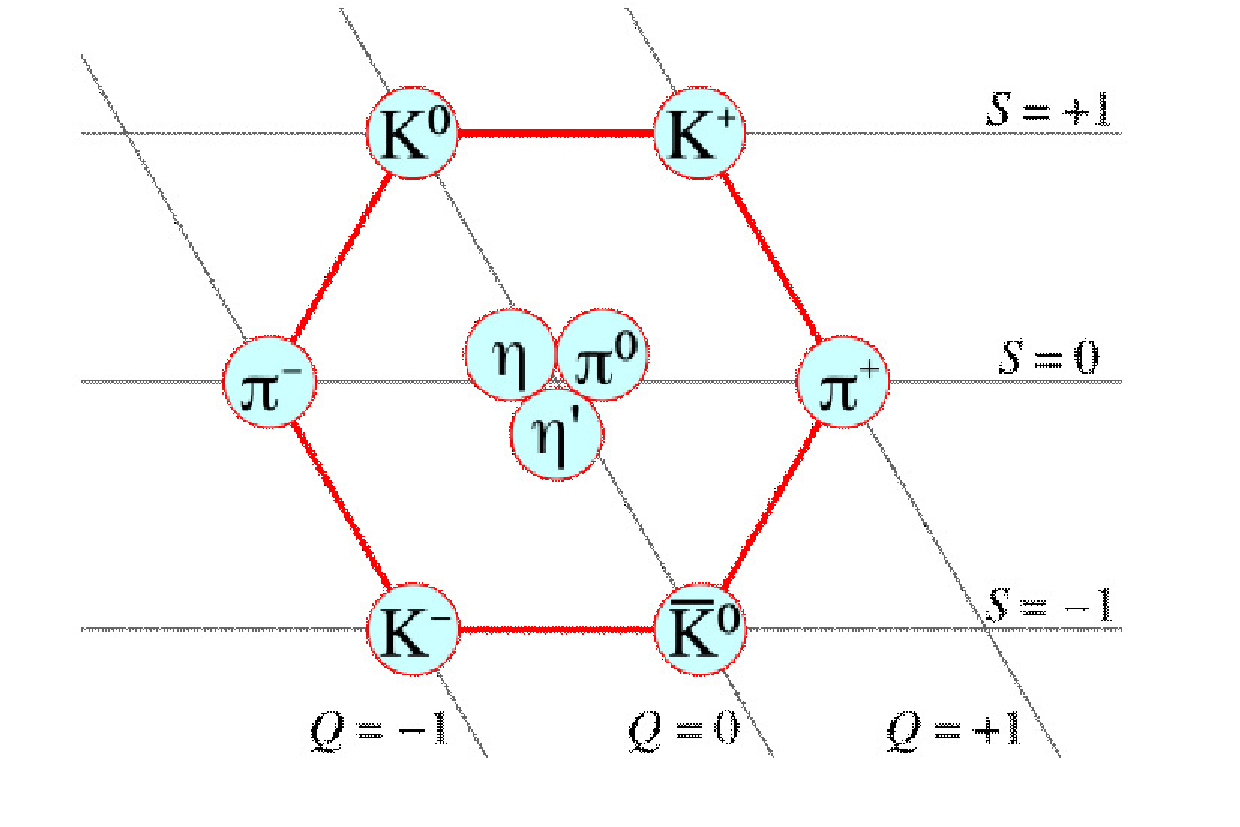
\includegraphics[width=0.65\columnwidth,height=0.5\qfigheight]{\grpath/intro/pseudoscalar.pdf}\label{fig:nonet.pseud}
%}
%
%\subfloat[Nonet of Vector Mesons][]{ %Feynman diagram of \piz Dalitz decay
%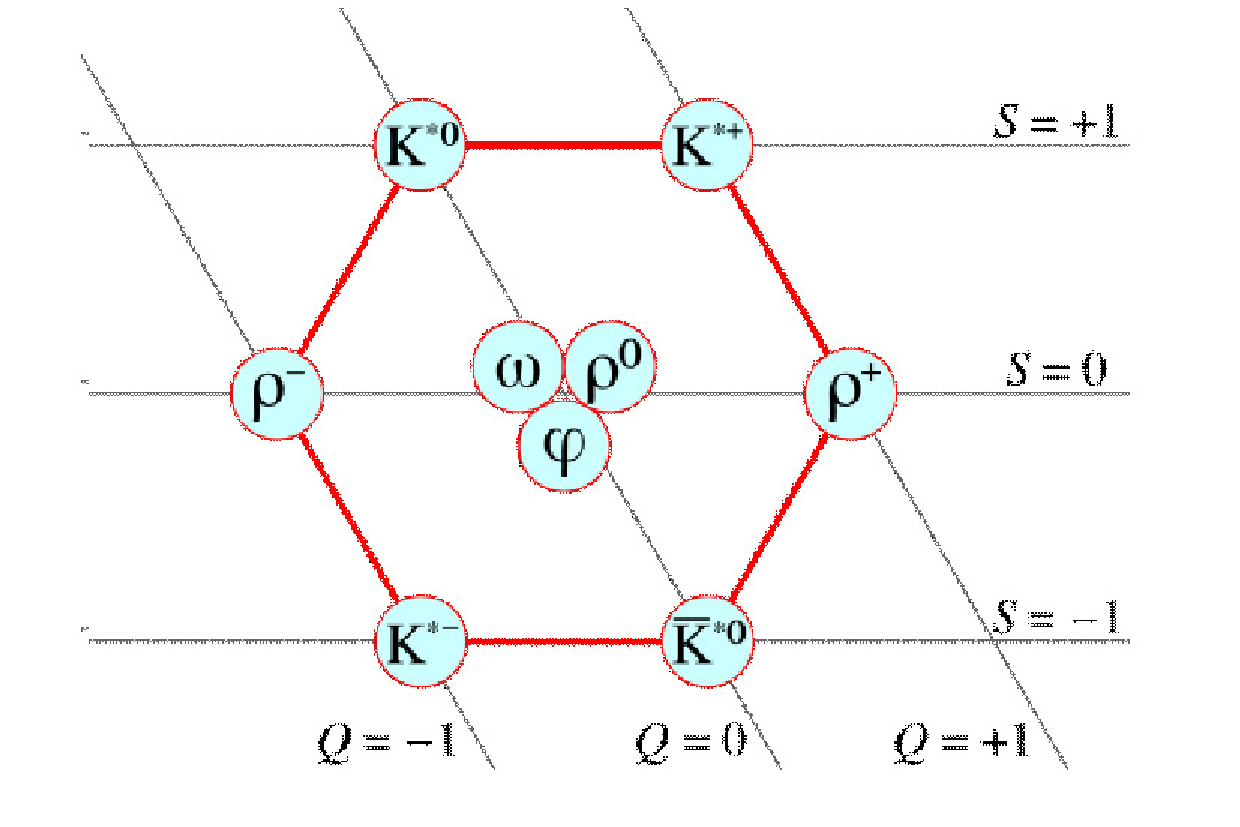
\includegraphics[width=0.65\columnwidth,height=0.5\qfigheight]{\grpath/intro/vector.pdf}\label{fig:nonet.vect}
%}
%\caption[Nonet of Pseudoscalar and Vector Mesons]{\label{fig:piz.alldecay}Nonet of pseudoscalar mesons~\subref{fig:nonet.pseud}. Nonet of vector mesons~\subref{fig:nonet.vect}.}
%
%\end{center}\end{figure}
%
%The \piz is the lightest meson with a mass of $m_{\pi^0}= (134.9766 \pm 0.0006) {\rm MeV}$ \cite{pdg2014}. The quark content is:
%\begin{equation}
% \pi^0 : \frac{1}{\sqrt{2}}\left(u \bar u  - d \bar d \right).
%\end{equation}

%In the intended analysis, it is planned to investigate the cross-section of the \piz.
